\documentclass{article}
\usepackage[utf8]{inputenc}
\usepackage{graphicx}
\usepackage{mathtools} 
\usepackage{textcomp}
\usepackage{titling}
\usepackage{subfig}
\usepackage{amsmath}
\usepackage[parfill]{parskip}
\usepackage{xcolor}
\definecolor{LightGray}{gray}{0.9}
\usepackage{titlesec}
\setcounter{secnumdepth}{4}
\usepackage[a4paper,left=1cm,right=1cm,top=1cm,bottom=1.5cm,]{geometry}
\usepackage{eqparbox}
\usepackage{enumitem}

\title{\vspace{-2cm} CS231N Assignment 1 - KNN}
\date{\vspace{-5ex}}

\begin{document}
\maketitle

\section{Intuition}
\subsection{Training and Prediction}
\begin{itemize}
    \item In training stage, KNN simply memorizes the training data (effectively a NOP operation)
    \item In prediction stage, for each \textbf{test} image KNN finds the \textit{nearest} training data (that it previously memorized) 
    \item As number of training samples approaches infinity, KNN can represent any function (subject to many technical conditions)
        \begin{itemize}
            \item However, this suffers from \textit{curse of dimensionality}
            \item For uniform coverage of training space, number of training points increases exponentially with dimension
        \end{itemize}
\end{itemize}

\subsection{Distance Metrics}
\begin{figure}[htp]
    \centering
    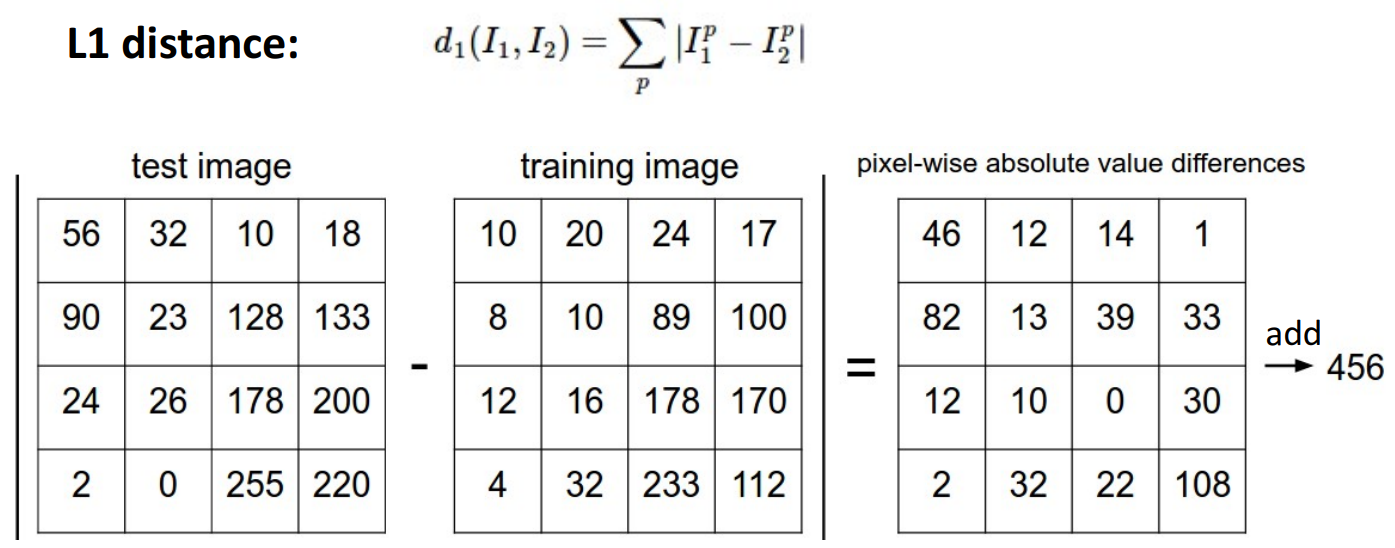
\includegraphics[width=12cm, scale=1]{images/L1_distance.PNG}
    \caption{}
\end{figure}

\begin{figure}[htp]
    \centering
    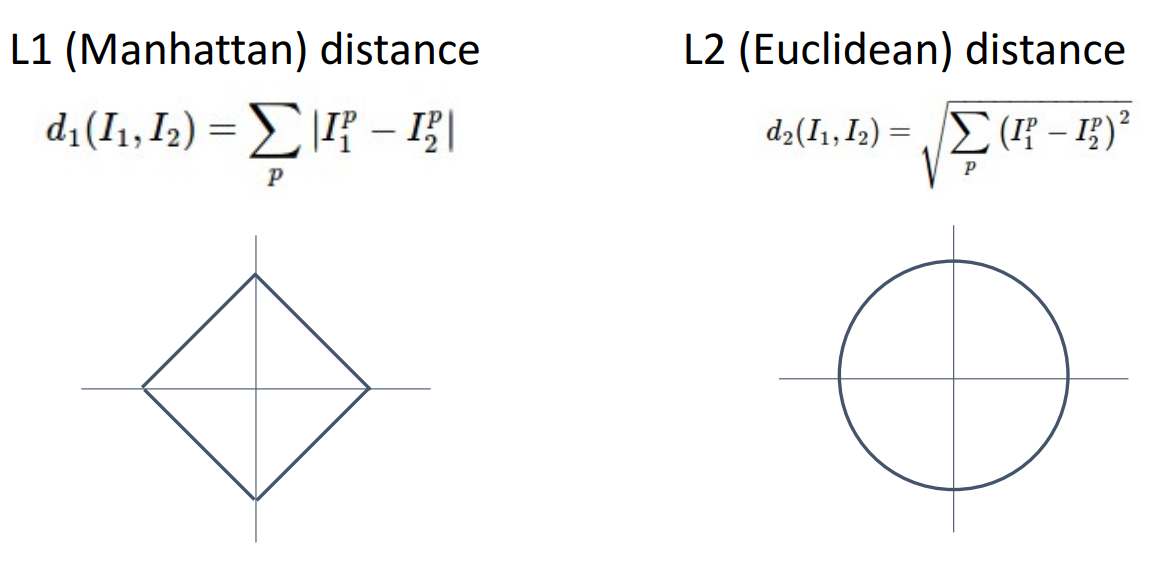
\includegraphics[width=12cm, scale=1]{images/L1_vs_L2_distance.PNG}
    \caption{}
\end{figure}


\section{Per-pixel calculations}
\begin{minipage}[c]{0.5\textwidth}
    \vspace{0pt}
    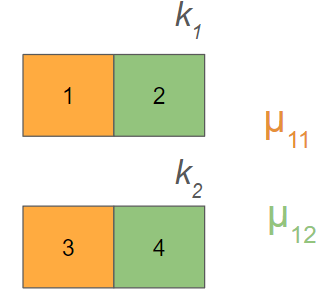
\includegraphics[width=4cm, scale=1]{images/knn_inlineQ2.PNG}
    \captionsetup{justification=centering}
    \captionof{figure}{$p^{(k_{1})}$ and $p^{(k_{2})}$}
\end{minipage}%
\begin{minipage}[c]{0.5\textwidth}
    \vspace{0pt}
    \begin{itemize}
        \item General mean $\mu = \frac{1+2+3+4}{1*2*2}$
        \vspace{0.5cm}
        \item Pixel-wise mean $\mu_{ij} = 
            \begin{bmatrix}
                \mu_{11} \\
                \mu_{12}
            \end{bmatrix} = 
            \begin{bmatrix}
                \frac{1+3}{2} \\
                \frac{2+4}{2}
            \end{bmatrix} = 
            \begin{bmatrix}
                2 \\
                3
            \end{bmatrix}$
    \end{itemize}
\end{minipage}

\section{L2 Distance - Fully vectorised}
\begin{equation*}
    \begin{split}
    d_{2}(A,B) & = \sqrt{\sum_{p}{(A_{p}-B_{p})^{2}}} \text{ ; Where $\boldsymbol{A}$ and $\boldsymbol{B}$ are vectors indexed via $p$} \\
               & = \sqrt{\sum_{p}\Bigl\{(A_{p})^{2} - 2(A_{p} \cdot B_{p}) + (B_{p})^{2}\Bigr\}} \\
               & = \sqrt{\Bigl\{\sum_{p}(A_{p})^{2}\Bigr\} -2\Bigl\{\sum_{p}(A_{p} \cdot B_{p}) \Bigr\} + \Bigl\{\sum_{p}(B_{p})^{2}\Bigr\}} \\
               & = \sqrt{\Bigl\{\sum_{p}(A_{p})^{2}\Bigr\} -2\Bigl\{ \boldsymbol{A}\boldsymbol{B}^{T} \Bigr\} + \Bigl\{\sum_{p}(B_{p})^{2}\Bigr\}} \\
               & = \sqrt{\Bigl\{\sum_{p}(A_{p})^{2}\Bigr\} + \Bigl\{\sum_{p}(B_{p})^{2}\Bigr\} -2\Bigl\{ \boldsymbol{A}\boldsymbol{B}^{T} \Bigr\} }
    \end{split}
\end{equation*}

\subsection{Context}
\begin{figure}[htp]
    \centering
    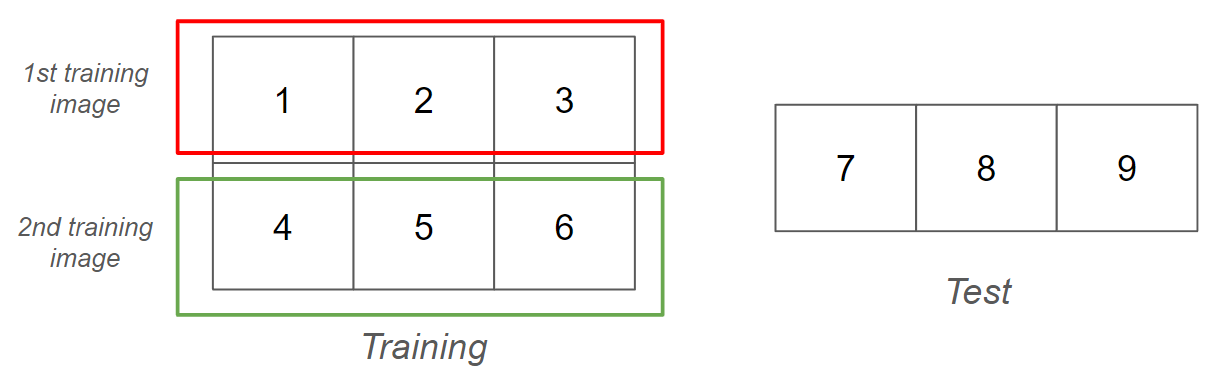
\includegraphics[width=12cm, scale=1]{images/knn_broadcast.PNG}
    \caption{}
\end{figure}
\begin{itemize}
    \item Training =  
            $\begin{bmatrix}
                1 & 2 & 3 \\
                4 & 5 & 6
            \end{bmatrix}$, 
          Test = 
            $\begin{bmatrix}
                7 & 8 & 9 \\
            \end{bmatrix}$
    \item We want to calculate the L2 distance between test image and every training image
\end{itemize}

\subsubsection{One loop}
\begin{enumerate}
    \item Broadcast; $(Tr-Te)_{broadcast} = 
            \begin{bmatrix}
                1-7 & 2-8 & 3-9 \\
                4-7 & 5-8 & 6-9
            \end{bmatrix} = 
            \begin{bmatrix}
                -6 & -6 & -6 \\
                -3 & -3 & -3
            \end{bmatrix}$ 
    \item Square terms; $(Tr-Te)_{broadcast}^{2} = 
            \begin{bmatrix}
                36 & 36 & 36 \\
                9 & 9 & 9
            \end{bmatrix}$
    \item Sum along rows; $\sum_{rows}(Tr-Te)_{broadcast}^{2} = 
            \begin{bmatrix}
                36+36+36 \\
                9+9+9
            \end{bmatrix} = 
            \begin{bmatrix}
                108 \\
                27
            \end{bmatrix}$
    \item Square root; $\sqrt{\sum_{rows}(Tr-Te)_{broadcast}^{2}} =
                            \begin{bmatrix}
                                \sqrt{108} \\
                                \sqrt{27}
                            \end{bmatrix}$
\end{enumerate}

\subsubsection{No loop}
\begin{enumerate}[label*=\arabic*.]
    \item Square \textbf {elements of} training matrix; $Tr_{squared} = 
            \begin{bmatrix}
                1 & 4 & 9 \\
                16 & 25 & 36
            \end{bmatrix}$
        \begin{enumerate}[label*=\arabic*.]
            \item $\sum_{row}Tr_{squared} = 
                    \begin{bmatrix}
                        1+4+9 \\
                        16+25+36
                    \end{bmatrix} = 
                    \begin{bmatrix}
                        14 \\
                        77
                    \end{bmatrix}$
        \end{enumerate}
    \item Square \textbf {elements of} test matrix; $Te_{squared} = 
            \begin{bmatrix}
                49 & 64 & 81
            \end{bmatrix}$
        \begin{enumerate}[label*=\arabic*.]
            \item $\sum_{row}Te_{squared} = 
                    \begin{bmatrix}
                        49+64+81
                    \end{bmatrix} = 
                    \begin{bmatrix}
                        194 \\
                    \end{bmatrix}$
        \end{enumerate}
    \item Broadcast; $\Bigl(\sum_{row}Tr_{squared} + \sum_{row}Te_{squared}\Bigr)_{broadcast} = 
                    \begin{bmatrix}
                        14 + 194 \\
                        77 + 194
                    \end{bmatrix} =
                    \begin{bmatrix}
                        208 \\
                        271
                    \end{bmatrix}$
    \item $2(\boldsymbol{Tr}\boldsymbol{Te}^{T}) = 
            2 \cdot \begin{bmatrix}
                        1 & 2 & 3 \\
                        4 & 5 & 6
                    \end{bmatrix}
                    \begin{bmatrix}
                        7 \\
                        8 \\
                        9
                    \end{bmatrix} = 
                    \begin{bmatrix}
                        100 \\
                        244
                    \end{bmatrix}$
    \item $\Bigl(\sum_{row}Tr_{squared} + \sum_{row}Te_{squared}\Bigr)_{broadcast} - 2(\boldsymbol{Tr}\boldsymbol{Te}^{T})$
\end{enumerate}



\end{document}